% Chapter 1

\chapter{Introduction and Motivation} % Main chapter title

\label{chapter1} % For referencing the chapter elsewhere, use \ref{Chapter1}

%----------------------------------------------------------------------------------------
The simultaneous localization and mapping (SLAM) problem questions the autonomy of a mobile robot in an unfamiliarised environment: would a robot be able to explore and incrementally construct the information of its surroundings, yet at the same time accurately locate its position in the complex, realistic environment?
Solutions to the SLAM problem would imply that a robot has become “truly autonomous” as it no longer requires arbitral instructions or fixed input in order to understand its relation with its situated context \cite{durrant2006simultaneous}.
Over the decades, multiple solutions have been proposed in different technical and mathematical forms, and have been applied to various fields of robots, including group aerial, underwater, indoor, etc. 
From a theoretical perspective, SLAM is deemed as a solved problem \cite{durrant2006simultaneous}. 

However, in a realistic environment, different solutions will showcase their advantages and disadvantages. 
For example, algorithms such as iterative closet point (ICP) perform exceptionally well in an indoor context, but when it comes to complex, outdoor environment, they may fail to reach the expectation for accuracy \cite{krinkin2018evaluation}. 
Moreover, substantial issue remains in implementing these solutions. 
Problems such as the trade-off between accuracy, speed, memory and power consumption continue to challenge the researchers and practical commercialization. 
Hence, there has been sustained research in practical implementation and evaluation of different SLAM solutions. 

In recent year, the creation of new sensors and increase in processing power have enabled the releases of newer, more accurate and efficient SLAM systems. 
As SLAM systems continue to evolve and develop, needs for evaluating diverse SLAM algorithms surge exponentially. 
Unfortunately, despite heated discussion over SLAM, there has been little attention devoted to standardizing the evaluation of all SLAM systems. 
Different approaches have been used by researchers to test and experiment the SLAM algorithms, making it difficult to compare the performance of various SLAM systems. 
Furthermore, most of the testing and evaluation can take considerable effort and have been done in a specific, manual procedure. 
Researchers need a plug and play system that can easily evaluate the performance different SLAM systems and streamline the testing process. 

Hence, SLAMBench has been created by numerous SLAM researchers to streamline and standardize the benchmarking process of SLAM systems. 
The program is structured to be dataset-agnostic and SLAM-system-agnostic, so that researchers can conveniently input their own SLAM model and testing data. 
In addition, by having a standard SLAM benchmarking program, researchers would also be able to rest assured that the quantitative testing results are reproducible \cite{bodin2018slambench2}. 
The program now is developed in multiple languages and supports eight state-of-the-art SLAM systems.

Yet, an essential component is missing in the current SLAMBenck software architecture: a real-time filter. 
While undoubtedly extracting as much information from sensors as possible would render the most accurate solution, fixed computational bounds and energy consuming limitation of a mobile robot will restrict the quantity and quality of sequential inputs that an algorithm can ingest \cite{strasdat2010real}. 
Therefore, before feeding the sensor data into the correspondence SLAM system, real-time preprocessing is an indispensable step to improve the computational speed and lower the energy consumption. 

\begin{figure}[h]
	\caption{Example of filtering in KinectFusion}
	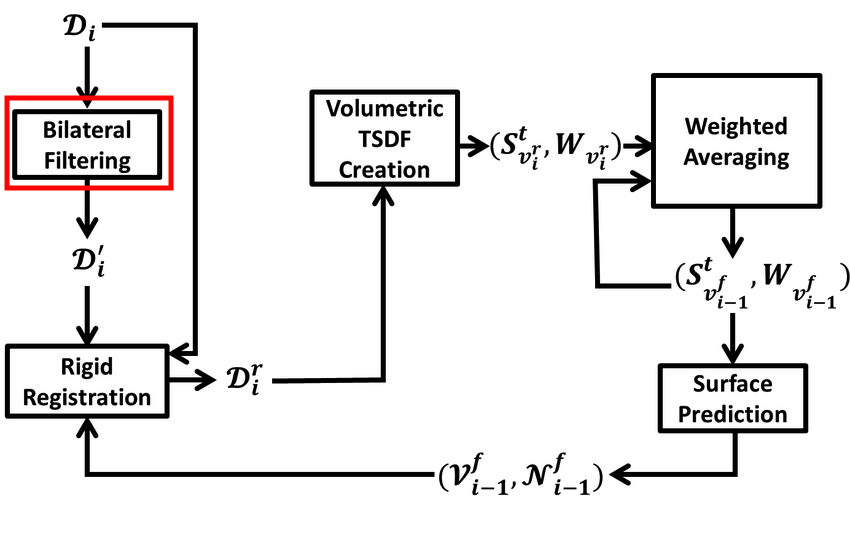
\includegraphics[width=11cm]{figures/kinectfusion.png}
	\centering
\end{figure}

Currently, the SLAMBench framework consists of two configurable parts – dataset and SLAM algorithms. 
To test the performance of filtering and other preprocessing method, researchers are forced to manually customized their filter with deliberate calibration, for which these tinkering approaches will defeat the purpose of SLAMBench and complicate the benchmarking process. 
In addition, current SLAMBench framework only allows one data pipeline to deliver sensor data sequentially from the I/O system, where data are ingested, to the loader, where the SLAM algorithms are evaluated. 
This simplistic design of data pipeline does not account for concurrent data delivery from multiple sensors and does not provide room for filtering and preprocessing multi-sensory data based on sequential time frames. 
Hence, restructuring the software architecture is required to decouple and modularize the new filtering module and ensure its compatibility with the rest parts of SLAMBench.

In this capstone project I introduce real-time filtering system for the current SLAMBench program. 
This filtering system enables researchers to evaluate the impact of various filtering and preprocessing techniques on different open source or proprietary SLAM systems. 
It is a tool that ensures the reproducibility of results for existing filtering methods and allows the integration and evaluation of new filters for SLAM algorithms. 
Through a series of testing and experimentations, we demonstrate its configurability, extensibility and its ease of use to benchmark different filters for SLAM systems. 
In summary, we present the following contributions:
\begin{itemize}
	\item A publicly available filtering system, integrated with SLAMBench, that supports quantitative, reproducible comparison of different filtering techniques for SLAM systems.
	\item A filtering system that is configurable, extensible and enables plug and play of new filters.
	\item Various experimenting cases of different filters (resize, blur, random drop, etc.) on state-of-art SLAM systems.
\end{itemize}